\documentclass{article}
\usepackage{amsmath, amssymb} % Required for math symbols and additional symbols
\usepackage[paper=letterpaper,
           hmargin={1in,1in},
           vmargin={1in,1in},
           ]{geometry}   % Allows you to change the margin sizes
\usepackage{enumitem}  % Required to re-label lists
\usepackage{tikz}      % Required for creating graphics

\title{Prep Work 17}
\author{Xander} 
\date{Apr 16}

\begin{document}

\maketitle
\noindent\textbf{Presentation:} 


%%%%%%%%%%%%%%%%% Don't delete anything above this line!
\section*{Exercise 6 4.4}  

Prove the chromatic number of any tree is two. Recall, a tree is a connected graph with no cycles.%

\begin{enumerate}[label= (\alph*)]
    \item Describe a procedure to color the tree below.
        \begin{center}
            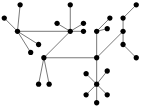
\includegraphics[width=0.8\linewidth]{Capture-2024-04-16-195919.png} % Adjust the path and filename as necessary
        \end{center}
    \item The chromatic number of \(C_n\) is two when \(n\) is even. What goes wrong when \(n\) is odd?
    \item Prove that your procedure from part (a) always works for any tree.
    \item Now, prove using induction that every tree has chromatic number 2.
\end{enumerate}
    

\vspace{0.5cm}
\noindent\textbf{Solution Draft:} 
\vspace{0.2cm}

\begin{enumerate}
    \item Start at one point, go to the next and switch colors, every other point connected to that once recieves the first color. Since this graph is a tree you will only need to use two colors
    \item When $n$ is odd, you will end up with two adjacent verticies of the same color since the cycles does not close evenly.
    \item The algorithm stated above will work for all trees.
    \item 

    \textbf{Base Case}
    For a single vertex tree, the algorithm works since you will only need once color.

    \textbf{Inductive Case}
    Assume every tree with $k$ verticies has a chromatic number of two. Consider a tree with $k+1$ verticies. By removing a leaf, you have a tree with $k$ verticies. No matter how many leafs you remove or add, the chromatic number will never change since it will never create a cycle.
\end{enumerate}

%%%%%%%%%%%%%%%%%%%
\section*{Exercise 10 4.4}  

Find the chromatic number of the graph below and prove you are correct.

\begin{center}
    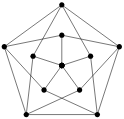
\includegraphics[width=0.8\linewidth]{Capture-2024-04-16-200146.png} % Adjust the path and filename as necessary
\end{center}


\vspace{0.5cm}
\noindent\textbf{Solution Draft:} 
\vspace{0.2cm}

The chromatic number of the graph below is 3. You cannot use less colors than 3.

\begin{center}
    \includegraphics[width=0.8\linewidth]{/Users/xander/Desktop/Screenshot 2024-04-16 at 20.10.49.png} % Adjust the path and filename as necessary
\end{center}


%%%%%%%%%%%%%%%%%%%%%%%%%%%%%%%%%%%%
\section*{Size of Infinite Sets Problem}  

Determine which of the following sets are countable and which are uncountable.
\begin{enumerate}
    \item[a.] $\{a, b, c\}$
    \item[b.] All odd numbers in $\mathbb{N}$
    \item[c.] $\mathbb{N}$
    \item[d.] $\mathbb{Z}$
    \item[e.] $\mathbb{R}$
\end{enumerate}

\vspace{0.5cm}
\noindent\textbf{Solution Draft:} 
\vspace{0.2cm}

\begin{enumerate}
    \item[a.] Countable 
    \item[b.] Countable
    \item[c.] Countable
    \item[d.] Countable
    \item[e.] Uncountable
\end{enumerate}

%%%%%%%%%%%%%%%%%%%%%%%%%%%%%%%%%%%%
\end{document}
